\documentclass{scrreprt}
\usepackage{listings}
\usepackage{underscore}
\usepackage{graphicx}
\usepackage[bookmarks=true]{hyperref}
\usepackage[utf8]{inputenc}
\usepackage[english]{babel}
\usepackage{float}
\usepackage{enumitem}
\setlist[itemize]{topsep=4pt, itemsep=4pt, parsep=0pt, partopsep=0pt}
\usepackage{pdflscape}
\usepackage{array}
\usepackage{tabularray}

\UseTblrLibrary{booktabs}
\DefTblrTemplate{firsthead,middlehead,lasthead}{default}{}

\DefTblrTemplate{firstfoot}{default}{
  \UseTblrTemplate{caption}{default}
}

\DefTblrTemplate{middlefoot}{default}{
  \UseTblrTemplate{capcont}{default}
}

\DefTblrTemplate{lastfoot}{default}{
  \UseTblrTemplate{caption}{default}
}

\usepackage[
    a4paper,
    left=2cm,
    right=2cm,
    top=3cm,
    bottom=3cm
]{geometry}


\hypersetup{
    bookmarks=false,    % show bookmarks bar?
    pdftitle={Attribute-Driven Design Document},    % title
    pdfauthor={Quach Gia Kiet},                     % author
    pdfsubject={ADD for Community Social Network LKForum},
    pdfkeywords={Website, ADD, Software Architecture},
    colorlinks=true,       % false: boxed links; true: colored links
    linkcolor=blue,       % color of internal links
    citecolor=black,       % color of links to bibliography
    filecolor=black,        % color of file links
    urlcolor=purple,        % color of external links
    linktoc=page            % only page is linked
}%
\def\myversion{1.4}
\date{}

\begin{document}

\begin{flushright}
    \rule{16cm}{5pt}\vskip1cm
    \begin{bfseries}
        \Huge{ATTRIBUTE-DRIVEN \\ DESIGN DOCUMENT}\\
        \vspace{1.5cm}
        for\\
        \vspace{1.5cm}
        LKFORUM WEBSITE\\
        \vspace{1.5cm}
        \LARGE{Version \myversion}\\
        \vspace{1.5cm}
        Prepared by : Quach Gia Kiet\\
        Vo An Khoi\\
        \vspace{1.5cm}
        Submitted to : Nguyen Trinh Dong \\Lecturer\\
        \vspace{1.5cm}
        \today\\
    \end{bfseries}
\end{flushright}

\tableofcontents

\chapter{Design Constraints}

\begin{itemize}[leftmargin=2cm]
    \item \textbf{Performance:} The system must deliver fast content browsing and responsive real-time interactions. It uses the \textbf{Go/Gin} framework for high-concurrency request handling, \textbf{Redis caching} to offload repetitive read queries, and an \textbf{Event-Driven} architecture using in-memory \textbf{Go Channels} for non-blocking background tasks.
    \item \textbf{Security:} The system must protect accounts, privileged operations, and private conversations. It uses \textbf{JSON Web Tokens (JWT)} for authentication, \textbf{Role-Based Access Control (RBAC)} for authorization, Redis-backed \textbf{rate limiting} for abuse prevention, and client-side encryption for private messaging.
    \item \textbf{Supportability:} The system must make incidents and sensitive actions traceable. It uses structured runtime logging with Go \texttt{slog} for diagnostics and a dedicated audit-log model for critical user, moderator, and administrator actions.
    \item \textbf{Manageability:} The system must expose operational signals that allow administrators and developers to check service health and observe runtime behavior. It provides \texttt{/health}, \texttt{/ready}, and Prometheus-compatible \texttt{/metrics} endpoints.
    \item \textbf{Maintainability:} The architecture must remain easy to modify as LKForum grows. It enforces a \textbf{Layered Architecture} (Routes, Controllers, Services, Repositories) and interface-based boundaries to keep business logic, transport logic, and data access isolated.
\end{itemize}

\chapter{Quality Attribute Requirements}

\section{Performance}

\subsection{High-Throughput Content Retrieval}
\begin{table}[H]
\centering
\begin{tblr}{
    width=\textwidth,
    hlines,
    vlines,
    rows = {valign=m},
    colspec = {Q[l,3.5cm] Q[l,11.5cm]}
}
\textbf{Element} & \textbf{Statement} \\
\textbf{Stimulus} & Thousands of users simultaneously request the global public feed. \\
\textbf{Stimulus source} & Guest Users, Members. \\
\textbf{Environment} & Peak usage times causing high read traffic. \\
\textbf{Artifact} & Post Service, Redis Cache Layer, MongoDB. \\
\textbf{Response} & The system serves feeds directly from Redis RAM using a Read-Through caching strategy, bypassing the database completely for cached endpoints. \\
\textbf{Response measure} & Database CPU utilization remains < 60\% during peak loads. >= 95\% of feed read requests process within 500ms. \\
\end{tblr}
\end{table}

\subsection{Asynchronous Processing}
\begin{table}[H]
\centering
\begin{tblr}{
    width=\textwidth,
    hlines,
    vlines,
    rows = {valign=m},
    colspec = {Q[l,3.5cm] Q[l,11.5cm]}
}
\textbf{Element} & \textbf{Statement} \\
\textbf{Stimulus} & A user publishes a new post that requires notifying hundreds of followers and updating analytics. \\
\textbf{Stimulus source} & Members. \\
\textbf{Environment} & Normal operation during content creation. \\
\textbf{Artifact} & Post Service, Notification Service, In-Memory Event Bus (Go Channels). \\
\textbf{Response} & The Post Service saves the content and immediately returns success to the user. It then asynchronously publishes an event to the Event Bus via Go Channels. Background goroutines consume the event and process notifications. \\
\textbf{Response measure} & The HTTP response time for post creation remains < 1 second, unaffected by the number of followers receiving notifications. \\
\end{tblr}
\end{table}

\section{Security}

\subsection{Authentication and Authorization}
\begin{table}[H]
\centering
\begin{tblr}{
    width=\textwidth,
    hlines,
    vlines,
    rows = {valign=m},
    colspec = {Q[l,3.5cm] Q[l,11.5cm]}
}
\textbf{Element} & \textbf{Statement} \\
\textbf{Stimulus} & Users attempt to access restricted API endpoints, such as deleting a post or changing community settings. \\
\textbf{Stimulus source} & Malicious Actors, Members, System Admins. \\
\textbf{Environment} & Normal operation over public internet. \\
\textbf{Artifact} & JWT Validation Middleware, RBAC Module. \\
\textbf{Response} & The system validates JWT signatures and strictly enforces RBAC rules. It checks if the authenticated user holds the required role (e.g., Moderator or Admin) before allowing the action. \\
\textbf{Response measure} & 100\% of unauthorized API requests are rejected with HTTP 403 Forbidden. \\
\end{tblr}
\end{table}

\subsection{Abuse Prevention with Rate Limiting}
\begin{table}[H]
\centering
\begin{tblr}{
    width=\textwidth,
    hlines,
    vlines,
    rows = {valign=m},
    colspec = {Q[l,3.5cm] Q[l,11.5cm]}
}
\textbf{Element} & \textbf{Statement} \\
\textbf{Stimulus} & A user or malicious actor repeatedly calls sensitive endpoints such as login, OTP verification, post creation, or report submission. \\
\textbf{Stimulus source} & Members, Guests, Malicious Actors. \\
\textbf{Environment} & Public internet during normal operation or abuse attempts. \\
\textbf{Artifact} & Redis Rate Limiting Middleware, Auth Routes, Post Routes. \\
\textbf{Response} & The system increments a Redis counter scoped by endpoint and client identifier. Requests within the configured limit proceed normally; requests above the limit are rejected before reaching business logic. \\
\textbf{Response measure} & Excessive requests are rejected with HTTP 429 Too Many Requests within the active rate-limit window. \\
\end{tblr}
\end{table}

\subsection{Data Privacy for Private Messaging}
\begin{table}[H]
\centering
\begin{tblr}{
    width=\textwidth,
    hlines,
    vlines,
    rows = {valign=m},
    colspec = {Q[l,3.5cm] Q[l,11.5cm]}
}
\textbf{Element} & \textbf{Statement} \\
\textbf{Stimulus} & Two members exchange private messages through a one-to-one conversation. \\
\textbf{Stimulus source} & Members. \\
\textbf{Environment} & Direct messaging via WebSocket connections. \\
\textbf{Artifact} & Client-side Cryptography Module (Svelte), WebSocket Service, Messaging Service, MongoDB. \\
\textbf{Response} & The sender's client encrypts the message before sending it to the backend. In the current implementation scope, an AES-GCM client-side prototype demonstrates the E2EE data path. The backend stores and routes only ciphertext, nonce, algorithm, and key version metadata. \\
\textbf{Response measure} & Private message plaintext is not stored in MongoDB; database records contain encrypted payload fields instead of readable message content. \\
\end{tblr}
\end{table}

\section{Supportability}

\subsection{Audit and User Activity Logging}
\begin{table}[H]
\centering
\begin{tblr}{
    width=\textwidth,
    hlines,
    vlines,
    rows = {valign=m},
    colspec = {Q[l,3.5cm] Q[l,11.5cm]}
}
\textbf{Element} & \textbf{Statement} \\
\textbf{Stimulus} & A system administrator needs to trace the action history of a suspected malicious user. \\
\textbf{Stimulus source} & System Administrators, Security Auditors. \\
\textbf{Environment} & Post-incident investigation. \\
\textbf{Artifact} & Audit Log Service, Audit Log Repository, MongoDB \texttt{audit\_logs} Collection. \\
\textbf{Response} & The system records a persistent audit entry for critical state-changing actions, including actor, role, action, target type, target identifier, reason, IP address, user agent, metadata, and timestamp. \\
\textbf{Response measure} & Critical authentication, moderation, report, ban, and unban actions are retrievable from the audit log collection for investigation. \\
\end{tblr}
\end{table}

\subsection{Structured Error Diagnostics with slog}
\begin{table}[H]
\centering
\begin{tblr}{
    width=\textwidth,
    hlines,
    vlines,
    rows = {valign=m},
    colspec = {Q[l,3.5cm] Q[l,11.5cm]}
}
\textbf{Element} & \textbf{Statement} \\
\textbf{Stimulus} & A user reports an unexpected HTTP 500 Internal Server Error when attempting to vote on a poll. \\
\textbf{Stimulus source} & Members. \\
\textbf{Environment} & Production environment during fault condition. \\
\textbf{Artifact} & Go \texttt{slog} Logger, Service Layer, Middleware Layer. \\
\textbf{Response} & The backend emits structured diagnostic logs with stable fields such as action, user id, target id, request path, and error details. User-facing responses remain generic when internal details are sensitive. \\
\textbf{Response measure} & Developers can identify the failing component and relevant context from structured logs without searching unstructured console output. \\
\end{tblr}
\end{table}

\section{Manageability}

\subsection{Health and Readiness Checks}
\begin{table}[H]
\centering
\begin{tblr}{
    width=\textwidth,
    hlines,
    vlines,
    rows = {valign=m},
    colspec = {Q[l,3.5cm] Q[l,11.5cm]}
}
\textbf{Element} & \textbf{Statement} \\
\textbf{Stimulus} & A developer or deployment environment needs to determine whether the backend process is alive and whether its required dependencies are reachable. \\
\textbf{Stimulus source} & Developers, Administrators, Deployment Environment. \\
\textbf{Environment} & Local development, staging, or production runtime. \\
\textbf{Artifact} & Go Backend, MongoDB Client, Redis Client, \texttt{/health} and \texttt{/ready} Endpoints. \\
\textbf{Response} & The backend exposes a liveness endpoint for process health and a readiness endpoint that checks MongoDB and Redis connectivity before reporting the service as ready. \\
\textbf{Response measure} & \texttt{/health} returns HTTP 200 when the process is alive; \texttt{/ready} returns dependency status for MongoDB and Redis. \\
\end{tblr}
\end{table}

\subsection{Runtime Metrics for Monitoring}
\begin{table}[H]
\centering
\begin{tblr}{
    width=\textwidth,
    hlines,
    vlines,
    rows = {valign=m},
    colspec = {Q[l,3.5cm] Q[l,11.5cm]}
}
\textbf{Element} & \textbf{Statement} \\
\textbf{Stimulus} & Developers and administrators need visibility into request volume, latency, cache behavior, WebSocket activity, message delivery, moderation decisions, and notification creation. \\
\textbf{Stimulus source} & Developers, Administrators. \\
\textbf{Environment} & Runtime operation under normal and peak usage. \\
\textbf{Artifact} & Metrics Middleware, Metrics Registry, Prometheus-compatible \texttt{/metrics} Endpoint, Prometheus Scrape Configuration. \\
\textbf{Response} & The backend records counters, gauges, and histograms and exposes them through a Prometheus-compatible endpoint. Prometheus can scrape the backend for operational analysis. \\
\textbf{Response measure} & Metrics such as HTTP request counts, request durations, feed cache hit/miss counts, active WebSocket connections, messages sent, and moderation decisions are visible from \texttt{/metrics}. \\
\end{tblr}
\end{table}

\section{Maintainability}

\subsection{Layered Architecture and Interface-Based Design}
\begin{table}[H]
\centering
\begin{tblr}{
    width=\textwidth,
    hlines,
    vlines,
    rows = {valign=m},
    colspec = {Q[l,3.5cm] Q[l,11.5cm]}
}
\textbf{Element} & \textbf{Statement} \\
\textbf{Stimulus} & A developer needs to add a new cross-cutting capability such as feed caching, rate limiting, audit logging, metrics, or private-message encryption support. \\
\textbf{Stimulus source} & Development Team. \\
\textbf{Environment} & Development and maintenance phases. \\
\textbf{Artifact} & Routes, Controllers, Services, Repositories, Interfaces, Bootstrap Wiring. \\
\textbf{Response} & The backend separates HTTP routing, request handling, business rules, data access, and infrastructure wiring. New capabilities can be introduced in the appropriate layer with limited changes to unrelated modules. \\
\textbf{Response measure} & Architectural changes remain localized to relevant routes, middleware, services, repositories, or platform packages instead of requiring broad rewrites across the codebase. \\
\end{tblr}
\end{table}

\chapter{Architectural Representation}

To describe the architecture of the LKForum System, the following views are presented:

\section{Logical View}
This view presents the system's modular decomposition into functional components and subsystems. It aligns with the \textbf{System Context} of the C4 model.

\begin{figure}[H]
    \centering
    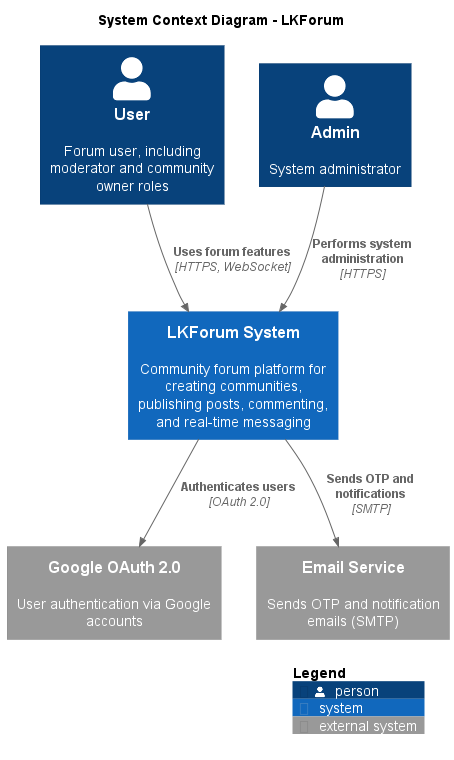
\includegraphics[width=0.9\textwidth]{diagrams/LKForum_System_Context.png}
    \caption{System Context Diagram}
\end{figure}

\begin{itemize}
    \item \textbf{Layered Architecture \& Interfaces:} The backend strictly separates concerns into Routes, Controllers, Services, and Repositories. Interfaces define contracts between layers (e.g., \texttt{PostService} interface), allowing for easy mock generation and unit testing.
    \item \textbf{IAM (Identity \& Access Management) Module:} Handles user registration, JWT-based stateless authentication, Google OAuth SSO integration, and RBAC.
    \item \textbf{Community \& Content Modules:} Manages the lifecycle of sub-forums, posts, and nested comments.
    \item \textbf{Event-Driven Hub:} An internal message bus utilizing \textbf{Go Channels and Goroutines} that decouples core business logic from auxiliary tasks (like firing push notifications or updating search indexes), ensuring high performance without relying on external message brokers.
    \item \textbf{Communication Module:} Facilitates real-time features including private messaging via WebSockets and client-side encrypted message payloads.
\end{itemize}

\section{Implementation View}
This view outlines the organization of code and deployment artifacts, aligning with the \textbf{Component Diagram} of the C4 model.

\begin{figure}[H]
    \centering
    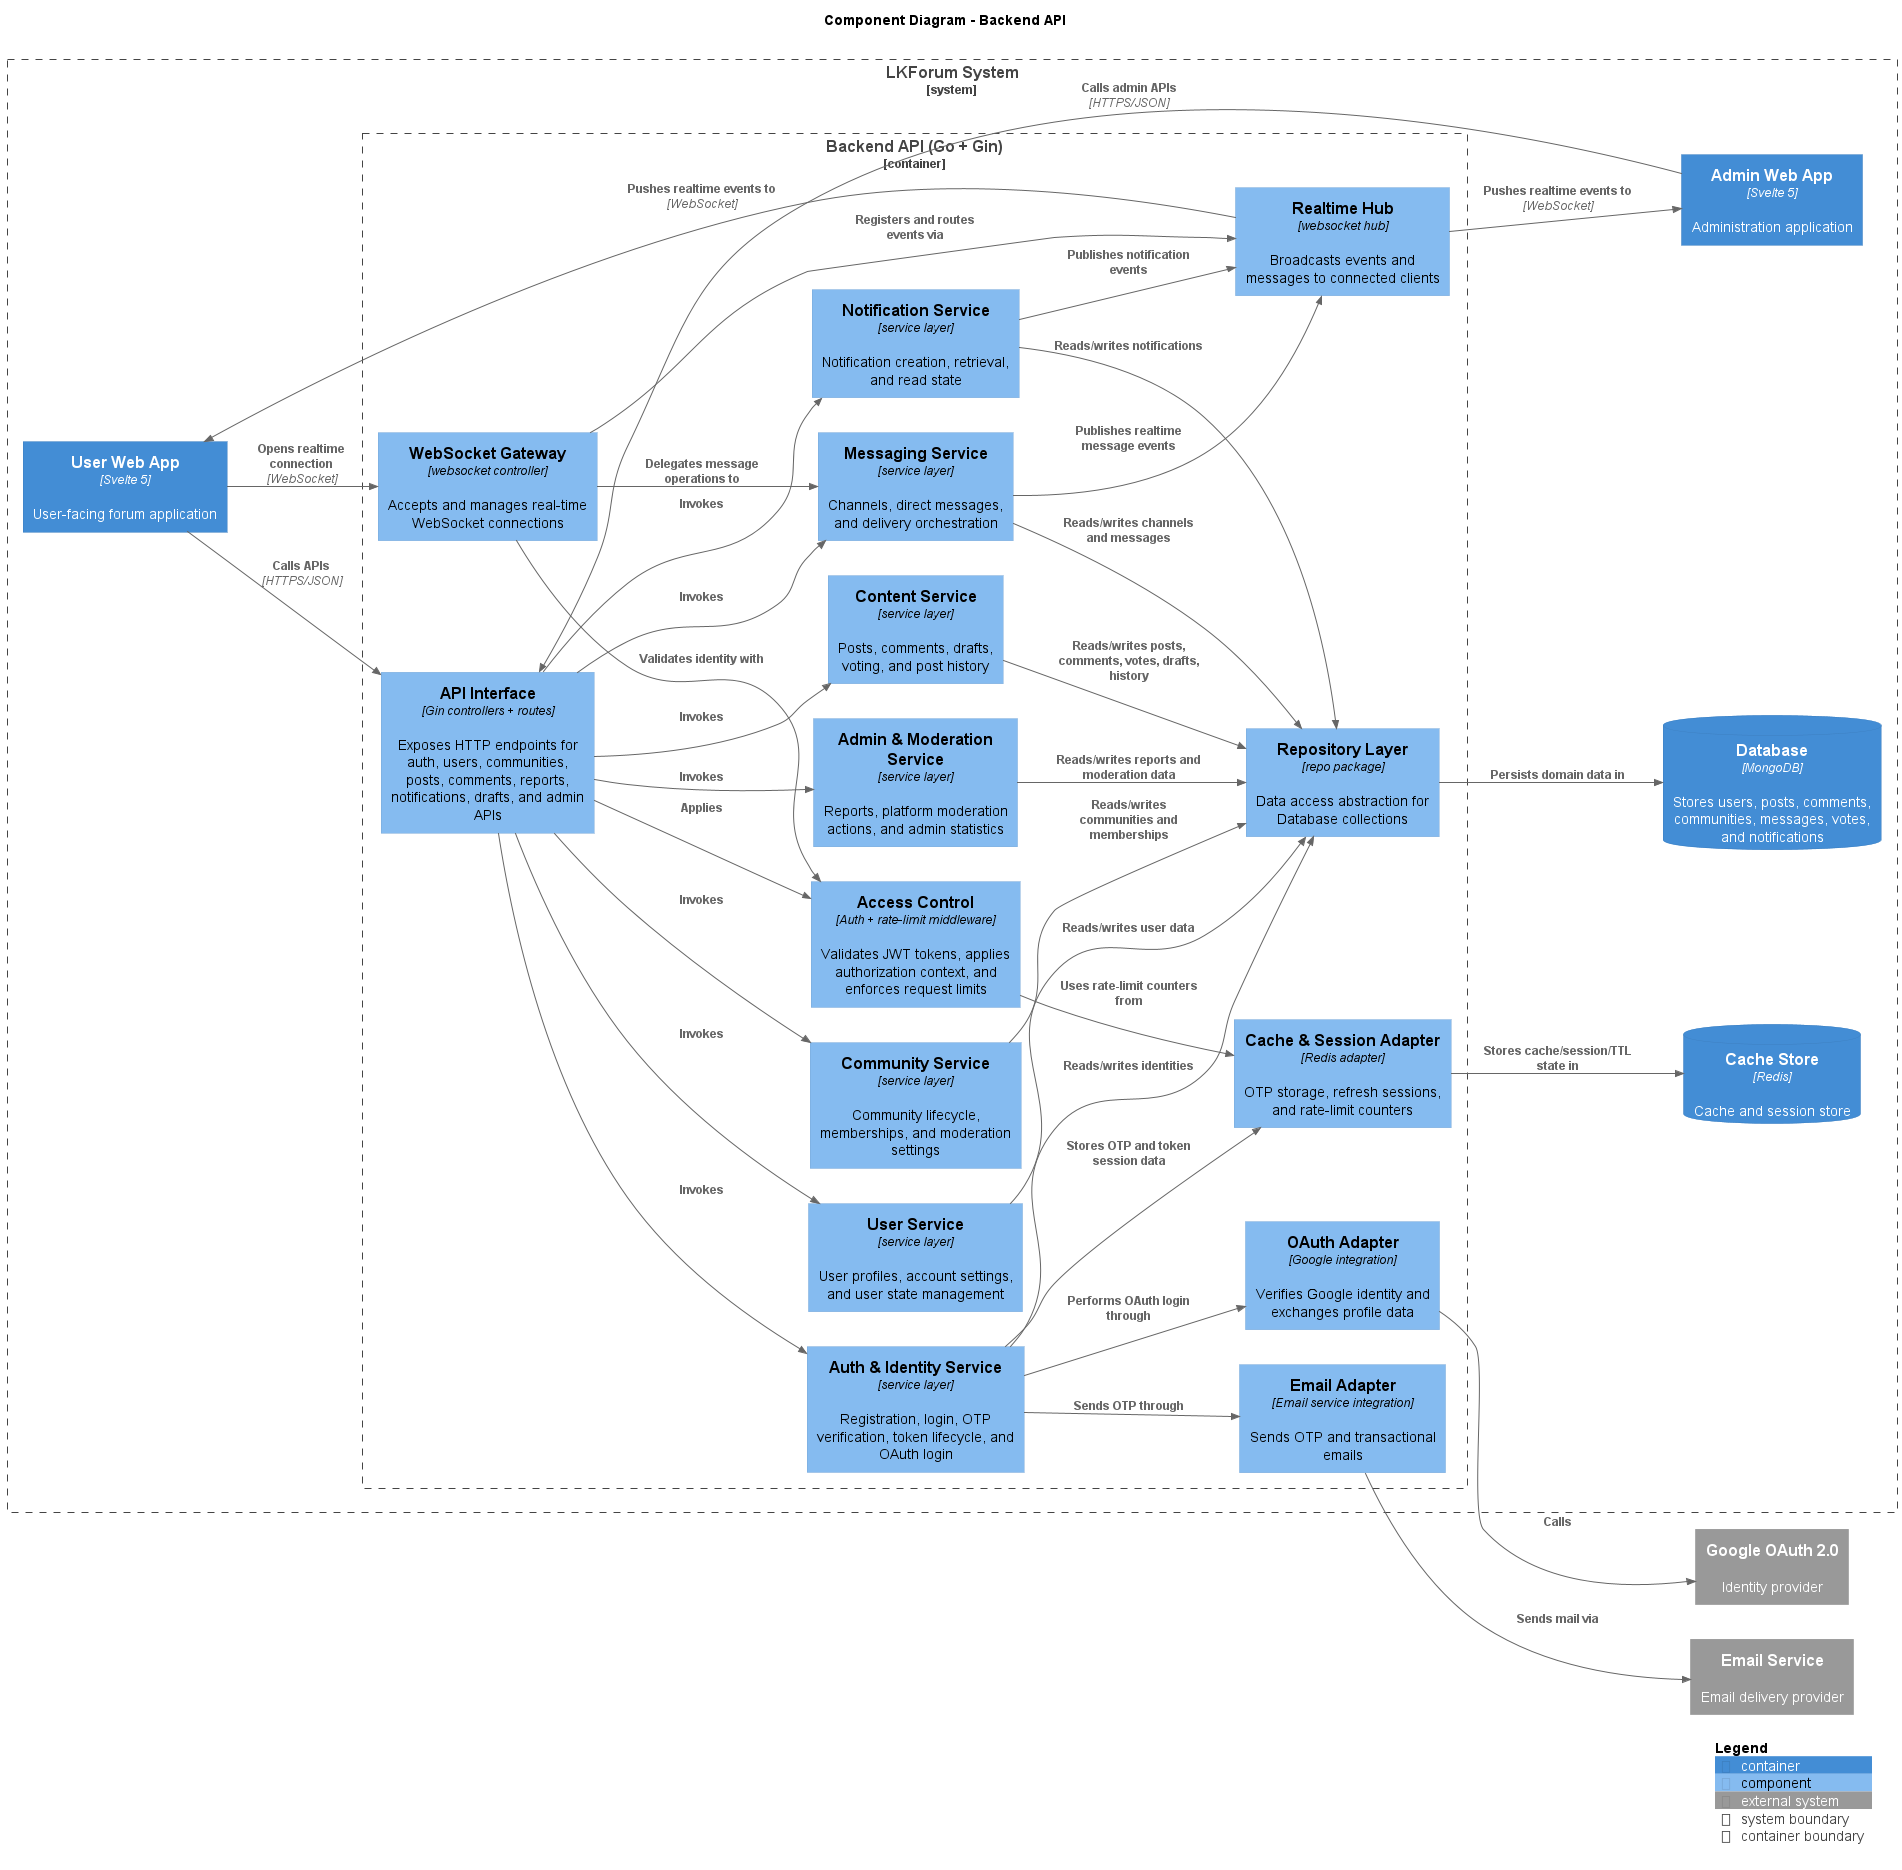
\includegraphics[width=0.9\textwidth]{diagrams/LKForum_Component_Backend.png}
    \caption{Backend Component Diagram}
\end{figure}

\begin{itemize}
    \item \textbf{Backend Organization:} The backend is a monolithic Go application exposing REST APIs and WebSocket endpoints. 
    \item \textbf{Frontend Organization:} Separated into two distinct SPAs built with Svelte and Vite:
    \begin{itemize}
        \item \texttt{user-web}: The main interface for Guests, Members, and Community Moderators.
        \item \texttt{admin-web}: A dedicated dashboard for System Administrators.
    \end{itemize}
    \item \textbf{Observability Implementation:} The backend exposes Prometheus-compatible metrics, readiness checks, and structured runtime logs using Go \texttt{slog}. Critical business actions are stored separately as audit-log records.
\end{itemize}

\section{Deployment View}
Describes the physical deployment and runtime environment of system components, aligning with the \textbf{Container Diagram} of the C4 model.

\begin{figure}[H]
    \centering
    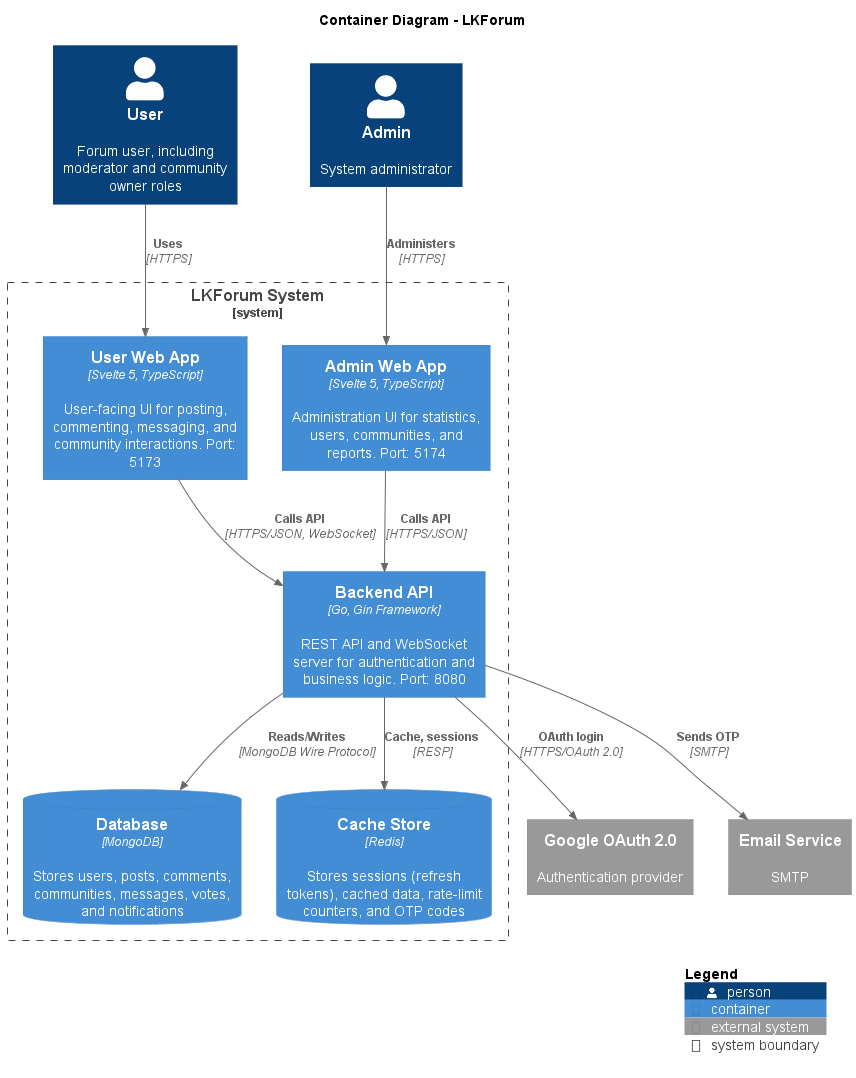
\includegraphics[width=0.9\textwidth]{diagrams/LKForum_Container.png}
    \caption{Container Diagram}
\end{figure}

\begin{itemize}
    \item \textbf{Containerization:} The entire ecosystem is containerized using Docker, avoiding the overhead of Kubernetes while maintaining isolation.
    \item \textbf{Orchestration:} A \texttt{docker-compose.yml} file manages the multi-container application network.
    \item \textbf{Node Layout:} 
    \begin{itemize}
        \item \textbf{Application Nodes:} Go Backend Container, User Web Frontend Container, Admin Web Frontend Container.
        \item \textbf{Data Nodes:} MongoDB container (persistent data), Redis container (caching).
        \item \textbf{Monitoring Nodes:} Prometheus container for scraping backend metrics.
    \end{itemize}
\end{itemize}

\section{Data View}
Focuses on data models, storage strategy, and external data integrations.

\begin{itemize}
    \item \textbf{Primary Storage (MongoDB):} Chosen for its flexible schema design, suitable for dynamic content types (polls, media arrays).
    \item \textbf{Caching (Redis):} Acts as an in-memory cache to absorb high read loads for public feeds, and stores fast-expiring data like session tokens and OTPs.
    \item \textbf{Secure Messaging Storage:} Private messages stored in MongoDB contain encrypted payload fields; the server routes them while client devices handle encryption and decryption in the current E2EE prototype.
\end{itemize}

\end{document}
